%%%%%%%%%%%%%%%%%%%%%%%%%%%
% IEEE Submission Dashboard - https://ieee.atyponrex.com/submission/dashboard
%%%%%%%%%%%%%%%%%%%%%%%%%%%

% IEEE Transactions on human--machine systems
% https://ieeexplore.ieee.org/xpl/mostRecentIssue.jsp?punumber=6221037

%---------------------------------------------------------------------
% \documentclass[10pt,journal,compsoc]{IEEEtran}
% \documentclass[lettersize,journal]{IEEEtran}
% \documentclass[letterpaper,journal]{IEEEtran}
\documentclass[journal]{IEEEtran}
% ==== Core packages (normalized) ====

% How to hide statements:
%   - To enable  tags: \iftrue  and \fi
%   - To disable tags: \iffalse and \fi
% How to turn-on (or turn-off) page number:
%   - To turn-on  the page number: {plain}
%   - To turn-off the page number: {empty}
% Usage (Syntax):
%   \documentstyle[twocolumn]{article}
%   \pagestyle{empty}
%    ...
%   \maketitle
%   \thispagestyle{empty}

% How to print the page number at each page
\pagestyle{empty}

\usepackage[T1]{fontenc}
\usepackage[utf8]{inputenc}
\usepackage{microtype}
\usepackage{amsmath,amssymb}
\usepackage{amsthm}  % theorem 환경을 사용하기 위한 필수 패키지
%\usepackage{amsmath}
%\usepackage{amssymb}
\usepackage{makecell}
%\usepackage{amsmath,amsfonts,amssymb,mathtools}
%\usepackage{amsthm}
\usepackage{graphicx}
\usepackage{booktabs}
\usepackage{siunitx}
\usepackage{xspace}
\usepackage{pifont}
% Checkmark / Xmark symbols
\newcommand{\cmark}{\ding{51}}
\newcommand{\xmark}{\ding{55}}

\usepackage{listings}
\usepackage{xcolor}
\usepackage{xurl}
\usepackage{url}

% Hyperlinks to content
% \usepackage[linktocpage=true]{hyperref}
% \usepackage{hyperref}
% \usepackage[nameinlink]{cleveref}
% \usepackage[hidelinks]{hyperref}
\usepackage[colorlinks=true,linkcolor=blue,citecolor=blue,urlcolor=black]{hyperref}

\usepackage{cleveref}
%\usepackage{amsmath,amsfonts}
% \usepackage{algorithmic}
\usepackage{algorithm}
\usepackage{array}
\usepackage[caption=false,font=normalsize,labelfont=sf,textfont=sf]{subfig}
\usepackage{textcomp}
\usepackage{stfloats}
\usepackage{verbatim}
\usepackage{cite}
%\hyphenation{op-tical net-works semi-conduc-tor IEEE-Xplore}
%\usepackage{amssymb,amsmath,amsthm,mathtools}
%\usepackage{hyphenat}

%% ------------- ORC ID Template: Start ----------------------
% https://tex.stackexchange.com/questions/498688/orcid-in-latex-file-of-ieee-trans-in-a-customized-position

\usepackage{scalerel}
\usepackage{tikz}
\usetikzlibrary{svg.path}

\definecolor{orcidlogocol}{HTML}{A6CE39}
\tikzset{
orcidlogo/.pic={
\fill[orcidlogocol] svg{M256,128c0,70.7-57.3,128-128,128C57.3,256,0,198.7,0,128C0,57.3,57.3,0,128,0C198.7,0,256,57.3,256,128z};
\fill[white] svg{M86.3,186.2H70.9V79.1h15.4v48.4V186.2z}
svg{M108.9,79.1h41.6c39.6,0,57,28.3,57,53.6c0,27.5-21.5,53.6-56.8,53.6h-41.8V79.1z M124.3,172.4h24.5c34.9,0,42.9-26.5,42.9-39.7c0-21.5-13.7-39.7-43.7-39.7h-23.7V172.4z}
svg{M88.7,56.8c0,5.5-4.5,10.1-10.1,10.1c-5.6,0-10.1-4.6-10.1-10.1c0-5.6,4.5-10.1,10.1-10.1C84.2,46.7,88.7,51.3,88.7,56.8z};
}
}

\newcommand\orcidicon[1]{\href{https://orcid.org/#1}{\mbox{\scalerel*{

\begin{tikzpicture}[yscale=-1,transform shape]
    \pic{orcidlogo};
\end{tikzpicture}
}{|}}}}

%% ------------- ORC ID Template: End ----------------------

\providecommand{\cmark}{\ding{51}}
\providecommand{\xmark}{\ding{55}}
\providecommand{\etal}{\textit{et al.}\xspace}
\DeclareMathOperator{\E}{\mathbb{E}}
\DeclareMathOperator{\Var}{\mathrm{Var}}

\theoremstyle{plain}
\newtheorem{theorem}{Theorem}[section]
\newtheorem{lemma}{Lemma}[section]
\newtheorem{corollary}{Corollary}[section]
\lstdefinelanguage{json}{
basicstyle=\ttfamily\small,
numbers=left,
numberstyle=\tiny,
stepnumber=1,
showstringspaces=false,
breaklines=true
}
\lstset{frame=single}
% === End patch ===

\IEEEoverridecommandlockouts

%####################################################### Geunsik Area ###########

\usepackage{algorithm}
\usepackage{algpseudocode}

% LaTeX에서 유니코드(①, ② 등)를 직접 사용
\usepackage{pifont}

% theorem, algorithm 가독성위해 디자인 개선
\usepackage[most]{tcolorbox}
\tcbuselibrary{listings}

%% To keep strictly tuned whitespace rules among sections (e.g., section, subsection, and subsubsection)
%% for decreasing or increasing the vertical space between sections
\usepackage{titlesec}
\titlespacing*{\section}{0.70pt}{0.50\baselineskip}{0.20\baselineskip}
\titlespacing*{\subsection}{0.70pt}{0.50\baselineskip}{0.20\baselineskip}
\titlespacing*{\subsubsection}{0.70pt}{0.50\baselineskip}{0.20\baselineskip}

%% Reduce vertical space (padding) after figure (a big effect)
%% Warning: "Text page 7 contains only floats."
%% https://www.reddit.com/r/LaTeX/comments/b4mipa/how_to_decrease_space_between_paragraph_and/
\setlength{\textfloatsep}{0.70pt}
\setlength{\abovecaptionskip}{0.70pt}
\setlength{\belowcaptionskip}{0.70pt}

\theoremstyle{definition}
\newtheorem{definition}{Definition}[section]
\urlstyle{tt}

\newcommand{\Lninetyfive}{L_{95}}
\newcommand{\Jain}{\mathcal{J}}
\providecommand{\cmark}{\ding{51}}
\providecommand{\xmark}{\ding{55}}

% JSON language for listings
\lstdefinelanguage{json}{
basicstyle=\ttfamily\small,
numbers=left, numberstyle=\tiny, stepnumber=1,
showstringspaces=false,
breaklines=true
}

% Listings setup (handles code blocks and JSON/diff-like listings)
\lstset{basicstyle=\ttfamily\small, breaklines=true, columns=fullflexible, showstringspaces=false}

% Minimal JSON language for listings
\lstdefinelanguage{json}{
basicstyle=\ttfamily\small,
showstringspaces=false,
morestring=[b]",
morecomment=[l]{//},
literate=
*{0}{{{\color{black}0}}}{1}
{1}{{{\color{black}1}}}{1}
{2}{{{\color{black}2}}}{1}
{3}{{{\color{black}3}}}{1}
{4}{{{\color{black}4}}}{1}
{5}{{{\color{black}5}}}{1}
{6}{{{\color{black}6}}}{1}
{7}{{{\color{black}7}}}{1}
{8}{{{\color{black}8}}}{1}
{9}{{{\color{black}9}}}{1}
{:}{{{\color{black}{:}}}}{1}
{,}{{{\color{black}{,}}}}{1}
{"}{{{\color{black}{"}}}}{1}
}

\begin{document}

    %----------------------------------------\input{./001-title}

    \title{From Alerts to Actions: A Human--AI Decision System for Reliable Action Execution Under Disaster Risk}

    %---------------------------------- \input{./003-author}

    \author{

    % for ORC-ID
    \IEEEauthorblockN{
    Geunsik Lim$^{\textsuperscript{\orcidicon{0000-0003-1845-7132}}}$
    }


    \thanks{G. Lim is with the Department of Electrical and Computer Engineering, Sungkyunkwan University, 2066, Seobu-ro, Jangan-gu, Suwon 16419, South Korea (e-mail: leemgs@g.skku.edu). }

    }

    % The paper headers
    % \markboth{Journal of \LaTeX\ Class Files,~Vol.~14, No.~8, August~2015}%
    % {Shell \MakeLowercase{\textit{et al.}}: Bare Demo of IEEEtran.cls for IEEE Transactions on Magnetics Journals}

    \markboth{IEEE Transactions on Consumer Electronics, Vol. 1, No. 1, May 2020}{G. Lim \MakeLowercase{\text
    {et al.}}: Thread Evolution Kit for Optimizing Thread Operations on IoT Devices}

    % make the title area
    \maketitle

    \thispagestyle{empty}%

    % -----------------------------\input{./005-abstract}
    \begin{abstract}
        Decision systems involving human and AI are being used in critical situations where inappropriate actions on the part of the human could result in serious consequences. Even though there has been an improvement in the predictive capabilities of AI, it does not automatically translate to appropriate actions on the part of the human. The focus of this paper is to understand how the structure of a human--AI decision system affects action execution, trust, and cognitive workload in uncertain situations.
        We introduce a new concept for human--AI decision system design: \emph{Action-Centered Human--AI Decision Framework (ACHDF)}, which focuses on action execution rather than on the performance of the algorithm.
        Our mixed-method evaluation strategy using controlled user studies ($n=52$), simulations of past disasters, and a pilot deployment in a municipality empirically shows the efficacy of ACHDF-based human--AI decision support systems in significantly outperforming a dashboard-based system in terms of action execution rates, response times, cognitive workload, trust, while avoiding technology overdependence.
        Our decision problems are not limited to disaster response but include a broader set of decision problems characterized by high levels of uncertainty, asymmetry in error costs, time pressure, and human accountability. Our work thus generalizes the human--machine system literature on human--AI decision support for reliable action execution.
    \end{abstract}

    \begin{IEEEkeywords}
        Human--AI decision systems, human-in-the-loop, trust calibration, cognitive workload, action execution
    \end{IEEEkeywords}

    %--------------------------------------- \input{./010-introduction}
\section{Introduction}
\IEEEPARstart{I}{n} fact, human--AI decision systems are being used in situations where there is high uncertainty, high consequence, and high speed \cite{Bach2024Access,PerezCerrolaza2024CSUR,Yang2022THMSReview}. These situations include healthcare triage, supervision of autonomous transportation systems, industrial safety systems, and emergency response systems \cite{Birkmann2013NatHazards,Sandoval2023IJDRS,Rokhideh2025IJDRS,Rao2024IJDRS,Charan2024,lim2026generativeaidrivenreliabilitylayer}. In these situations, artificial intelligence is being used to enhance the ability to predict situations accurately. However, human--machine systems research has consistently demonstrated that predictions do not always lead to human action \cite{Lai2023FAccT,Muller2022CHIWORK,Hodgson2013THMS}. In disaster contexts, effective response further depends on community-level coordination, resilient communications, and distributed sensing and reporting pipelines \cite{Stephens2022SIGDOC,Longo2025PMC,Yang2005MobiHoc}.
Decision making under conditions of uncertainty is an important aspect of human--machine systems research \cite{Yang2022THMSReview,Bach2024Access,lim2026generativeaidrivenreliabilitylayer}. When there is incomplete or uncertain information, human operators are required to consider risk, confidence, and responsibility in situations where they interact with machines. Previous research has demonstrated the fundamental influence of conditions of uncertainty on human action. In the context of AI systems, conditions of uncertainty are often not well communicated or are implicit \cite{McAllister2017IJCAI,Weidinger2022FAccT,Miller2019XRDS}.

In many systems, the results of an AI's computation are displayed as a set of probabilities or as an alarm, but often without adequate support for how these probabilities should guide action \cite{Miller2019XRDS,Bach2024Access}. Ultimately, it is left to the human to close the loop between prediction and action, and often in situations of cognitive stress \cite{Hodgson2013THMS,Zhang2022THMS}. A further important question is how human--AI systems can be designed for decision-making under uncertainty \cite{Lai2023FAccT}.
Machine learning advances have greatly enhanced the accuracy of predictions for a broad range of applications \cite{Mai2024TOS,PerezCerrolaza2024CSUR}. However, human factors research has also suggested that accuracy does not necessarily translate into human performance \cite{Lai2023FAccT,Yang2022THMSReview}. For example, humans might wait for confirmation before acting, or might choose not to follow an AI's advice when it is not trusted, or might become overly reliant on an AI when its accuracy is overstated \cite{Hodgson2013THMS,Raji2019AIES,Raji2022CACM}.
This illustrates one of the important shortcomings associated with prediction-focused system design approaches. The execution of human actions not only depends on what the system predicts but also on how the prediction is communicated and how the system provides control to the user. Without specific tools to address issues like trust calibration, workload management, and human override, there is a risk that the system could exacerbate automation bias or cognitive workload, thus negating the benefits of the system~\cite{Duan2014KDD,Hodgson2013THMS,Zhang2022THMS,Bach2024Access}.

While there has been extensive research on issues like automation, trust, and decision-making, there is a lack of empirical research on how specific human--AI system design decisions influence measurable action execution outcomes. The evaluation of most human--AI systems has been conducted on the basis of their prediction accuracy or usability, not on how well the system enables the human to execute appropriate actions under uncertain conditions \cite{Lai2023FAccT,Muller2022CHIWORK,Yang2022THMSReview,lim2026generativeaidrivenreliabilitylayer}.
This paper aims to address the following research question:
\begin{quote}
    \emph{How can a human--AI decision system be designed to reliably support timely and appropriate human action under conditions of high uncertainty?}
\end{quote}
In order to answer this question, we will examine how uncertainty-aware risk estimation, guardrailed AI recommendations, and human-in-the-loop escalation mechanisms impact action execution, trust calibration, and cognitive workload \cite{McAllister2017IJCAI,Weidinger2022FAccT,Assaad2023TAS,Miller2019XRDS}.
The main contributions of this paper to the research on human--machine systems include the following: First, we define \emph{action execution} as an important outcome variable for evaluating AI-assisted decision systems, going beyond accuracy as the primary measure for evaluating AI systems \cite{Lai2023FAccT,Yang2022THMSReview}. Second, we introduce a human--AI decision architecture that incorporates uncertainty, constraints on AI recommendations through guardrails, and human-in-the-loop escalation and override capabilities \cite{Assaad2023TAS,Bach2024Access}. Third, we conduct an empirical evaluation of our design and find its benefits for human action execution, cognitive workload, and trust calibration in a high-stakes decision task \cite{Bach2024Access,PerezCerrolaza2024CSUR}.

In addition to contributing to the body of knowledge in terms of specific results, this study also adds to the overall body of knowledge in human--machine systems by extending previous research in trust calibration, automation biases, and function allocation. Most notably, this study provides an empirical link between uncertainty-aware function allocation and human action execution in a way that can have significant effects on decision-making in high-stakes situations. This study seeks to address a long-standing gap between human factors theory and the practical design of human--AI systems \cite{Yang2022THMSReview,Hodgson2013THMS,Lai2023FAccT}.


    %----------------------------- \input{./020-related_work}
\section{Related Work}
In this section, we will discuss previous work that is related to the topic of human--AI decision systems, with a focus on the effects of automated decision support on the decision-making process of humans, trust in decision systems, and the execution of behavior in critical domains \cite{Bach2024Access,PerezCerrolaza2024CSUR,Yang2022THMSReview,Lai2023FAccT}. We will structure the previous work around three related research streams.


\subsection{Information Fusion and Network-Based Situational Awareness}
Many high-stakes decisions in disaster response are mediated by information ecosystems that combine heterogeneous sensor streams, ad hoc communications, and rapidly evolving social information. Resilience and early-warning systems often rely on wireless sensor networks and distributed reporting, where security and robustness are necessary to preserve actionable signal quality under disruption \cite{Yang2005MobiHoc}. Beyond physical sensors, post-disaster response may also incorporate opportunistic proximity-based data collection and community reporting, which can improve resource allocation and coordination under severe infrastructure constraints \cite{Longo2025PMC,Stephens2022SIGDOC}.
Network-analytic methods such as community detection provide one mechanism for structuring these large, noisy information environments. Prior work has examined scalable and model-based community discovery, resolution limits, and benchmark generation for large graphs \cite{Wakita2007WWW,Prokhorenkova2019WWW,Xian2025WWW,Slota2019SC,Sun2014FSKD,Rezaei2015ASONAM,Akhter2022ICCA}. Related studies have investigated overlapping and fuzzy community structure, which is useful when actors, organizations, and communication channels participate in multiple simultaneous operational groups \cite{Sun2011InformationSciences,Havens2013TFUZZ,Vehlow2013TVCG,Zhang2012KDD,Cao2020ICIIP,Li2022AppliedIntelligence}. While these graph-mining methods are not a core focus of our decision framework, they motivate how diverse upstream information sources can be structured and summarized so that downstream human--AI decision support can remain action-oriented under time pressure \cite{Duan2014KDD}.

\subsection{Human--Machine Decision Support Systems}
The human-machine decision support systems were widely researched in the context of supervisory control, command and control systems, and complex socio-technical systems \cite{Hodgson2013THMS,Yang2022THMSReview,Bach2024Access}. The research in this domain initially focused on the potential of automation in supporting human decisions in terms of enhancing the speed and consistency of information processing and the potential dangers of misallocating functions between humans and automation systems \cite{Hodgson2013THMS,Zhang2022THMS}.
More recent research has highlighted the importance of not only the quality of decision support information, but also the manner in which recommendations are incorporated into human decision-making processes \cite{Lai2023FAccT,Muller2022CHIWORK}. Systems that are limited to information display or prediction may place the burden of interpretation and decision-making on the human user, especially in time-critical situations \cite{Bach2024Access,PerezCerrolaza2024CSUR}. Recent research, therefore, suggests the need for decision support systems that go beyond information display to provide actionable recommendations while maintaining human control and responsibility \cite{Assaad2023TAS,Yang2022THMSReview}.

\subsection{Trust, Workload, and Automation Bias}
Trust and cognitive workload are important constructs used to explain the performance of human--machine systems \cite{Hodgson2013THMS,Bach2024Access}. Trust has been used to explain the extent to which users of decision support systems, for example, utilize the support, ignore the support, or misuse the support \cite{Lai2023FAccT,Yang2022THMSReview}. Previous research has demonstrated the negative effects of over-trust and under-trust on the performance of decision support systems, with over-trust leading to automation bias, thereby failing to detect errors, and under-trust leading to the failure to utilize decision support systems, thereby increasing workload \cite{Raji2019AIES,Raji2022CACM}.

Automation bias has been demonstrated to result when decision support systems provide recommendations but fail to represent their uncertainty \cite{Raji2019AIES,Weidinger2022FAccT}. On the other hand, the representation of uncertainty and the opportunity for humans to verify decisions has been demonstrated to increase trust levels \cite{Miller2019XRDS,Bach2024Access}. Similarly, the role of workload, as measured by the NASA Task Load Index (NASA--TLX), has been demonstrated to mediate the relationship between automation and performance \cite{Hodgson2013THMS,Yang2022THMSReview}. Decision support systems that reduce information processing and action selection can be used to reduce workload and increase the speed of responses by humans \cite{Lai2023FAccT,Muller2022CHIWORK}.

\subsection{AI Assistance in High-Stakes Environments}
In high-stakes environments such as healthcare, aviation, and emergency management, AI-assisted decision systems are being increasingly employed to facilitate time-critical decisions \cite{PerezCerrolaza2024CSUR,Bach2024Access,Rokhideh2025IJDRS,Rao2024IJDRS}. Although machine learning has helped improve the predictive accuracy of AI systems in such environments, empirical studies have demonstrated that the predictive ability of AI does not guarantee better human performance \cite{Lai2023FAccT,Yang2022THMSReview}.

Recent studies on responsible and explainable AI have emphasized the importance of human-in-the-loop controls and governance structures in AI development, particularly in safety-critical applications \cite{Weidinger2022FAccT,Assaad2023TAS,Miller2019XRDS,PerezCerrolaza2024CSUR}. However, most studies are either conceptual or algorithm-centric and do not investigate human behavioral outcomes. There has been limited empirical research on the impact of specific AI system designs such as uncertainty-aware escalation and guardrails on the execution of actions by humans \cite{Bach2024Access,Lai2023FAccT}.

By integrating these research streams, this research aims to place human action execution as a key criterion in the evaluation of AI-assisted decision systems and provide empirical contributions to the development of human-centered AI architectures that enhance their performance in high-stakes settings \cite{Yang2022THMSReview,Bach2024Access}.


%-----------------------------input{./050-design}

    \begin{figure}[t]
        \centering
        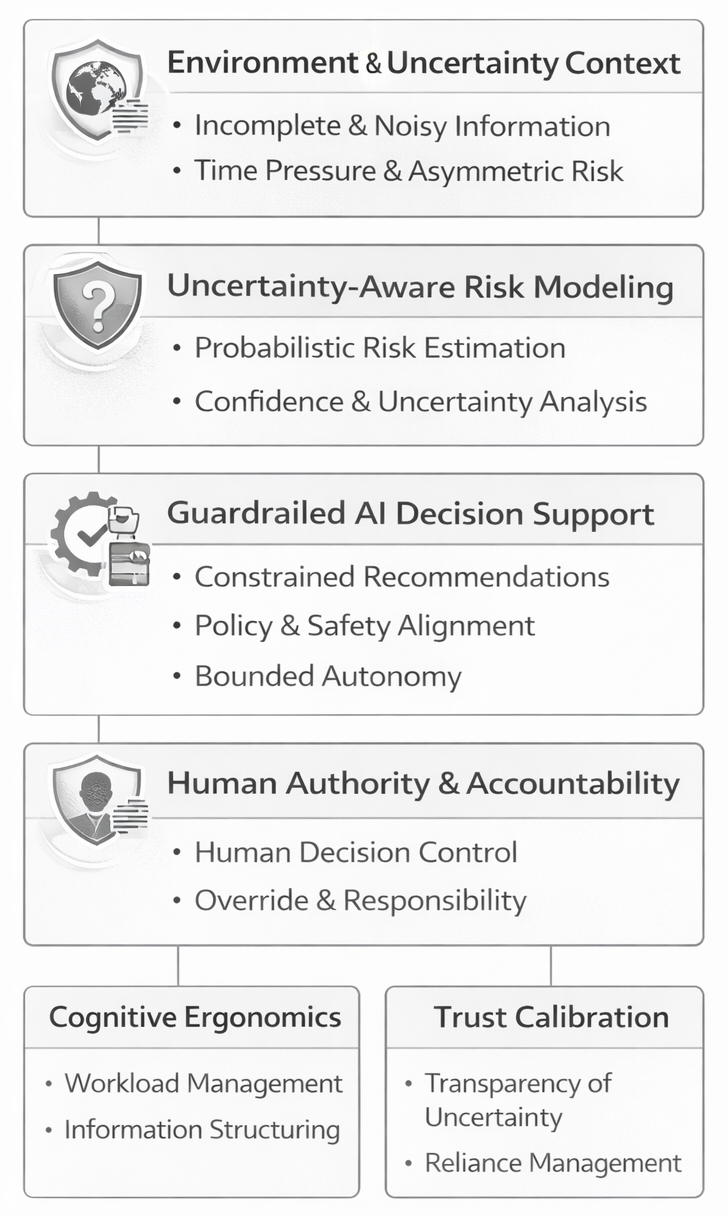
\includegraphics[width=0.60\linewidth]{fig_achdf_concept.png}
        \caption{Conceptual design layers of the Action-Centered Human--AI Decision Framework (ACHDF).
The framework structures human--AI decision support into four layered components: environment and uncertainty context, uncertainty-aware risk modeling, guardrailed AI decision support, and preserved human authority and accountability. Trust calibration and cognitive ergonomics operate as cross-cutting design considerations that influence interaction quality and reliable action execution under uncertainty.}
        \label{fig:achdf_concept}
    \end{figure}

    \begin{figure}[t]
        \centering
        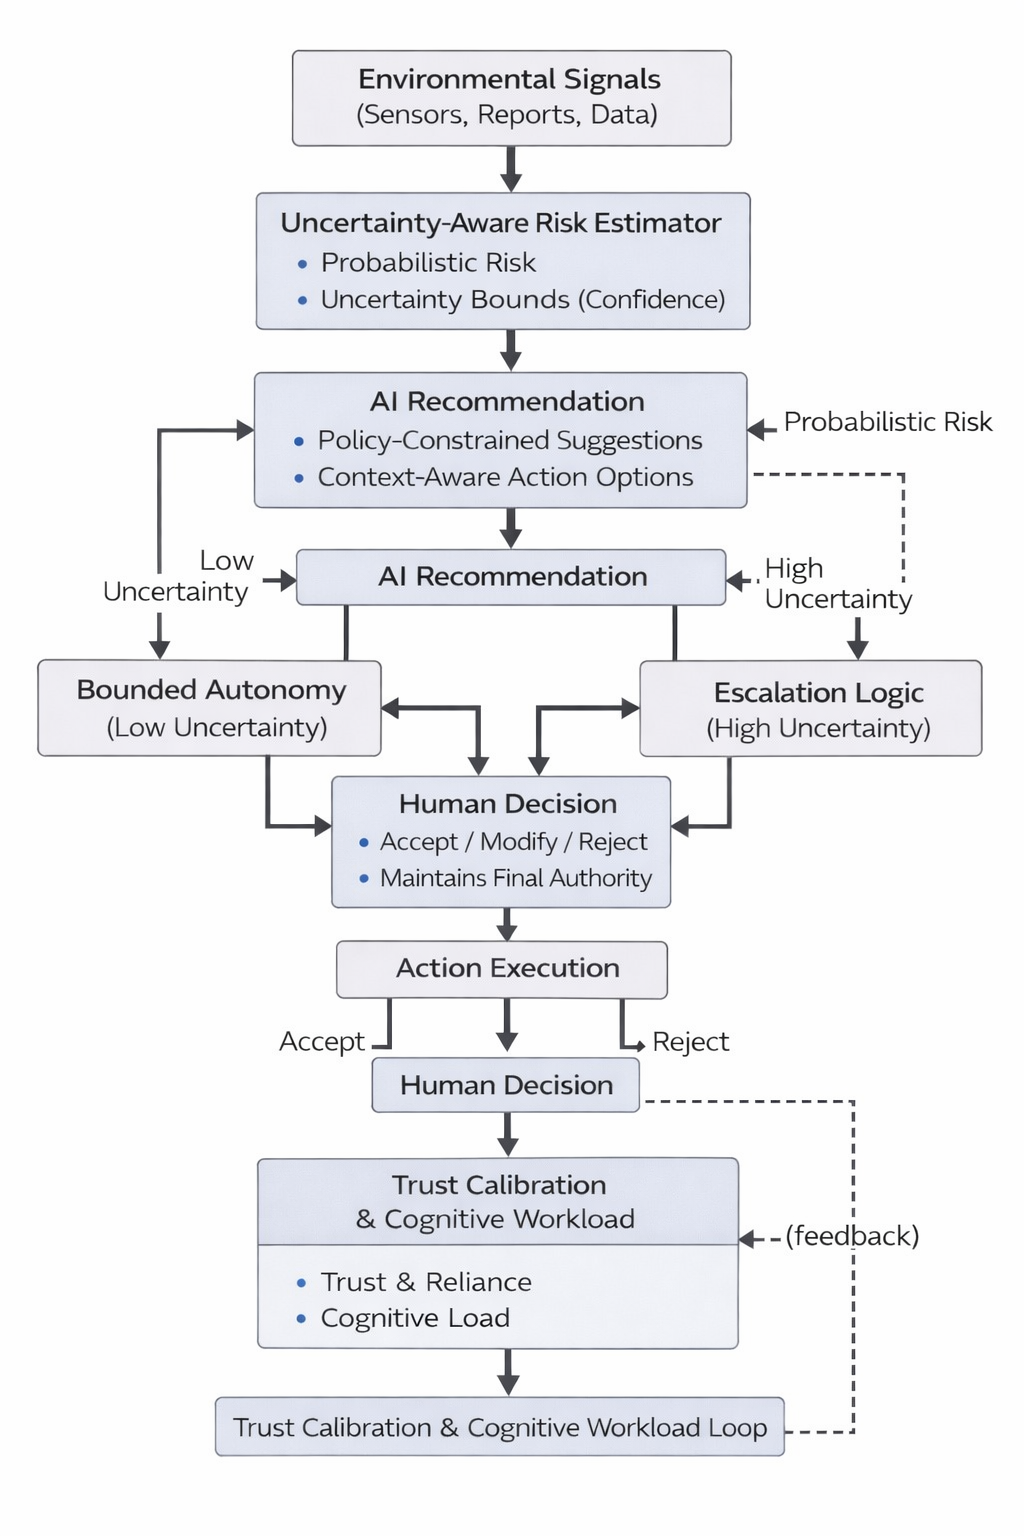
\includegraphics[width=0.95\linewidth]{fig_system_overview.png}
        \caption{Operational workflow of the proposed human--AI decision system.
Uncertainty-aware function allocation dynamically shifts decision authority between bounded autonomy and human-in-the-loop escalation.}
        \label{fig:system_overview}
    \end{figure}

    \section{System Overview and Architecture}
    This section is intended to introduce the proposed human--AI decision system. In addition, it is intended to introduce the architectural elements of the proposed human--AI decision system. The proposed human--AI decision system is intended to be non-autonomous and human-centric. It is intended to have a balanced approach to human and algorithmic decision-making. The architectural elements of the proposed human--AI decision system are based on the \textbf{Action-Centered Human--AI Decision Framework (ACHDF)}. In the proposed framework, there is a significant emphasis on human action execution as the primary goal of the system.

    A conceptual overview of the proposed action-centered architecture is illustrated in Fig.~\ref{fig:achdf_concept}. 
As shown in the figure, ACHDF is organized into four primary design layers. The \emph{environment and uncertainty context} layer captures incomplete, time-pressured, and asymmetric risk conditions that characterize high-stakes decision ecologies. Built on top of this, the \emph{uncertainty-aware risk modeling} layer produces probabilistic risk estimates together with explicit confidence and uncertainty bounds. These estimates are then translated into constrained, policy-aligned options within the \emph{guardrailed AI decision support} layer, which ensures that generated recommendations remain consistent with operational and safety constraints. Finally, the \emph{human authority and accountability} layer preserves human control through oversight, override, and responsibility mechanisms. The two cross-cutting elements shown at the bottom of the figure—trust calibration and cognitive ergonomics—continuously shape how information is presented so that operators can act reliably under uncertainty.

The dynamic operationalization of these layers in real-time decision making is depicted in Fig.~\ref{fig:system_overview}. 
This workflow view emphasizes how uncertainty-aware function allocation governs the interaction loop between AI and the human operator. When model confidence is high and risk is bounded, the system can provide tightly scoped, action-oriented recommendations under bounded autonomy. As uncertainty or potential impact increases, the escalation logic routes decisions to a human-in-the-loop review process, where the operator can approve, modify, or reject the suggested action. The feedback paths shown in the figure highlight how action outcomes and operator responses contribute to ongoing trust calibration and workload management, forming a closed human--AI decision loop oriented toward reliable action execution rather than mere prediction display.

    \subsection{Design Goals and Human-in-the-Loop Principles}
    The design of the proposed system is informed by three key goals that are derived from the fundamental principles of ACHDF. 
    
    \textbf{Goal 1 — Enabling Human Action Execution.}
    The proposed system must be able to support \emph{human action execution} effectively, as opposed to simply improving situational awareness and prediction accuracy. The key goal of the proposed system is therefore to enable effective human decision-making and action in operational settings.

    \textbf{Goal 2 — Supporting Calibrated Trust.}
    The proposed system must support appropriate trust calibration by making its uncertainty, model limitations, and potential failure modes explicit. By doing so, the proposed system enables users to develop a realistic understanding of when to trust the system's outputs and when to trust human judgment.

    \textbf{Goal 3 - Preserving Human Authority.}
    The system shall ensure the preservation of human authority in high-risk decisions by incorporating human-in-the-loop mechanisms and bounded autonomy. This means that, in safety-critical or ethically critical situations, the system will ensure that human operators have the final decision-making authority, avoiding over-reliance on automation or artificial intelligence.

    To ensure that these goals are achieved, the system will employ a human--AI collaboration paradigm, where the AI will be used to provide decision scaffolding and action-oriented recommendations, and the human will have the final responsibility for executing actions. The system will employ automation that assists in information synthesis and option generation, but will not be used for executing irreversible actions. This ensures the implementation of the concept of uncertainty-governed function allocation, where the level of automation will be dynamically adapted according to the level of uncertainty and criticality of actions.

    \subsection{Probabilistic Risk Estimation With Uncertainty}
    The heart of the system is a probabilistic risk estimation module that provides calibrated risk assessments along with uncertainty representations. Unlike many models that produce point estimate results, the model provides posterior risk distributions that include data-driven variability and epistemic uncertainty.

    \textbf{Role 1 in ACHDF.}
    These estimates of uncertainty are a crucial part of the decision logic. The risk level is interpreted in conjunction with the confidence intervals to determine whether the system should make recommendations on its own or whether the process should be deferred to humans. The system’s explicit representation of its own uncertainties helps to prevent the propagation of false precision and supports the reasoning of the risk level in a way that mirrors the human decision-making process.

    \subsection{Guardrailed AI Recommendation Module}
    To make risk estimates actionable and provide appropriate recommendations, a generative AI module is used by the system.

    \textbf{Role 2 in ACHDF}
    The system is constrained by a number of layers of structural guardrails that provide assurance with regard to reliability, consistency, and compliance with policies. These guardrails ensure that the recommendations generated by the system align with the risk estimates that were made previously and that there is no contradiction with those estimates.
    There are also further constraints that restrict the scope of recommendations based on operational and safety considerations. These recommendations also provide context cues that indicate the criticality and confidence levels associated with them, thereby avoiding information processing and facilitating a smooth transition to decisions and actions under pressure.
    By bounding the generative results within a structured decision process, the system harnesses the flexibility of generative AI while also limiting the risks of hallucination and overgeneralization, thereby ensuring that AI support is assistive rather than prescriptive.
    \begin{algorithm}[t]
        \caption{Uncertainty-aware escalation and human override policy}
        \label{alg:escalation}
        \begin{algorithmic}[1]
            \Require risk estimate $r$, uncertainty $u$, action criticality $c$
            \Require thresholds $\tau_r, \tau_u, \tau_c$
            \State $\textsc{mode} \leftarrow \text{``assist''}$
            \If{$u \ge \tau_u$ \textbf{or} $c \ge \tau_c$}
            \State $\textsc{mode} \leftarrow \text{``escalate''}$ \Comment{route to human review}
            \ElsIf{$r \ge \tau_r$}
            \State $\textsc{mode} \leftarrow \text{``recommend''}$
            \Else
            \State $\textsc{mode} \leftarrow \text{``monitor''}$
            \EndIf
            \If{$\textsc{mode} = \text{``escalate''}$}
            \State Present evidence and options to operator
            \State Operator selects: approve / modify / reject
            \Else
            \State Generate bounded recommendation via guardrails
            \EndIf
            \State Log decision context and outcome for audit and calibration
        \end{algorithmic}
    \end{algorithm}
    
\subsection{Human Override and Escalation Mechanisms}
The escalation process, as described in Algorithm~\ref{alg:escalation}, is linked to an uncertainty-aware policy that is used to dynamically allocate authority depending on the level of uncertainty and the criticality of the actions taken. The human override and escalation mechanism is an important part of the overall system architecture.
The system automatically escalates decisions to human operators if the level of uncertainty is above certain thresholds, the potential impact of the recommendation is high, and if certain policy constraints are violated. In fact, escalation is not a failure mode but a decision to escalate to ensure accountability under uncertain conditions.
The operators are free to either accept, modify, or reject the decision recommended by the AI system, and all of these operations are recorded for accountability purposes. This minimization of processing of superfluous information is also beneficial for the management of cognitive workload for time-critical situations.
This dynamic allocation of autonomy allows the system to offer effective assistance in regular situations and, at the same time, allow human control in uncertain or risky situations, thus striking a proper balance between performance and safety, as per the existing design principles for human--machine systems, which provides a platform for the ACHDF design principles proposed later in the paper.

\begin{table*}[t]
\centering
\caption{Transferability of ACHDF Design Principles Across Decision Ecologies}
\label{tab:achdf_transferability}
\begin{tabular}{p{3cm} p{3.2cm} p{3.2cm} p{2.8cm} p{3.9cm}}
\hline
\textbf{Decision Domain} &
\textbf{Primary Sources of Uncertainty} &
\textbf{Asymmetry of Error Costs} &
\textbf{Time Pressure Characteristics} &
\textbf{Role of Uncertainty-Aware Function Allocation} \\
\hline
Disaster Response &
Incomplete situational awareness, noisy sensor and report data, rapidly evolving conditions &
Delayed action leads to loss of life or property; false alarms incur operational cost &
Severe time pressure with dynamic escalation requirements &
AI provides bounded, action-oriented recommendations under low uncertainty; high uncertainty triggers human-in-the-loop escalation to preserve accountability \\

Autonomous Driving Supervision &
Perception uncertainty, rare edge cases, environment variability &
False negatives may cause accidents; false positives reduce efficiency and trust &
Sub-second to seconds-level response requirements &
Low-uncertainty situations allow bounded autonomy; ambiguous or novel situations escalate to human supervision and override \\

Medical AI (Triage / Diagnosis) &
Incomplete patient data, population-to-individual generalization limits &
False negatives risk patient harm; false positives cause overtreatment &
Moderate to high time pressure depending on clinical context &
AI assists with risk stratification and option generation; high uncertainty or high criticality decisions defer to clinicians \\

Military Safety Automation &
Adversarial uncertainty, incomplete intelligence, strategic deception &
Incorrect action may cause catastrophic or irreversible consequences &
High time pressure combined with strategic deliberation &
AI supports sensemaking and constrained recommendations; final decision authority remains with human operators under uncertainty \\

\hline
\end{tabular}
\end{table*}


\subsection{ACHDF Transferability Across Decision Ecologies}
Although the system architecture is instantiated and verified in the context of disaster response, the design principles are not domain-specific in nature. On the contrary, the architecture presented here is more aligned with a general class of \emph{decision ecologies} that are characterized by high uncertainty, asymmetrical costs of errors, timing pressures, and human accountability. The \textbf{Action-Centered Human--AI Decision Framework (ACHDF)} is intended to be more general in nature to cover a range of different safety-critical domains that have similar structural characteristics.

In order to further illustrate the general nature of the design principles presented in this work, Table \ref{tab:achdf_transferability} provides a decision ecology mapping that illustrates the transferability of the design principles to different application domains that are presented in this paper, such as the supervision of autonomous driving, medical AI in the context of medical triage or diagnostic support systems, or military safety automation systems. Despite the varying nature of the uncertainty in each of the application domains considered in this paper, the role of uncertainty-aware function allocation is similar in nature.
The contribution of this work is not about optimizing any particular domain or application scenario in the context of human--AI decisions under uncertainty.

    % -------------------------------\input{./060-evaluation}
    \section{Experimental Design and Methods}

    In this section, we describe the design of the experiments that can be used to test the proposed human--AI decision system. In our case, we aimed to isolate the effect of AI support on human action execution, response behavior, and subjective experience. In general, our design of experiments follows the usual practice of designing experiments to evaluate human--machine systems, where experiments are defined with clear conditions for baseline and treatment cases.

    \subsection{Study Design and Conditions (Baseline vs.\ AI-Assisted)}

    A within-subjects design was employed in the experiment. In this design, the participants are presented with the same decision-making task in two different conditions: a \emph{baseline} condition and an \emph{AI-assisted} condition. In the baseline condition, the participants were presented with the conventional dashboard-based interface. In the AI-assisted condition, the participants were presented with the proposed system that provides context-aware recommendations through the human--AI decision architecture.
    To avoid learning effects and order effects in the experiment, the presentation order of the two conditions is counterbalanced. The significance of the results is determined by conducting a paired test.
    In both the baseline and AI-assisted conditions, the same data is used. Hence, the difference in the performance between the two conditions is solely due to the presence of AI assistance.

    \subsection{Participants and Sampling Strategy}

    The demographics of participants are presented in Table~\ref{tab:participants}.

    \begin{table}[t]

        \caption{Participant Demographics}

        \label{tab:participants}

        \centering

        \begin{tabular}{l c}

            \hline

            Characteristic & Value \\

            \hline

            Total participants & 52 \\

            Age range & 20--50s \\

            Gender & Mixed \\

            Technical background & Low--High \\

            Study design & Within-subjects \\

            \hline

        \end{tabular}

    \end{table}

    The total number of participants recruited for the study was 52 in number. For the purpose of this study, participants were recruited using the stratified sampling technique in order to create diversity in terms of age, gender, and technical know-how. This technique has been selected due to the heterogeneity observed in operators in real-world decision environments.

    All participants gave their informed consent prior to the experiment. Although participants were not required to have prior knowledge in the domain area, training on the task interface was provided to all participants to create uniformity in terms of familiarity with the procedures.

    \subsection{Task Design and Procedure}

    The participants were required to complete a set of time-sensitive decision tasks. These tasks involved understanding risk information and making a decision on whether or not to take a protective action. These decision tasks were aimed at capturing the essential aspects of a high-stakes decision situation. These aspects include changes in information, uncertainty, and unbalanced error costs.
    The experiment involved a training period, and after that, the participants completed the task execution of both the experimental conditions. The participants were required to focus on the efficacy of the action rather than on the analysis of the information. The system was used to record the decision processes and interaction of the participants.

    \begin{table}[t]
        \caption{Outcome measures used in the controlled study}
        \label{tab:measures}
        \centering
        \begin{tabular}{p{0.23\linewidth}p{0.70\linewidth}}
            \toprule
            \textbf{Measure} & \textbf{Operationalization} \\
            \midrule
            Response Latency & Time from presentation of actionable information to action execution. \\
            Cognitive Workload & NASA--TLX overall score and subscales (post-condition). \\
            Trust & Post-task Likert-type items on perceived reliability, predictability, and appropriateness of recommendations. \\
            Usability & Standard usability scale (post-condition). \\
            \bottomrule
        \end{tabular}
    \end{table}

    %------------------------------------------------------

    \begin{figure}[t]
        \centering
        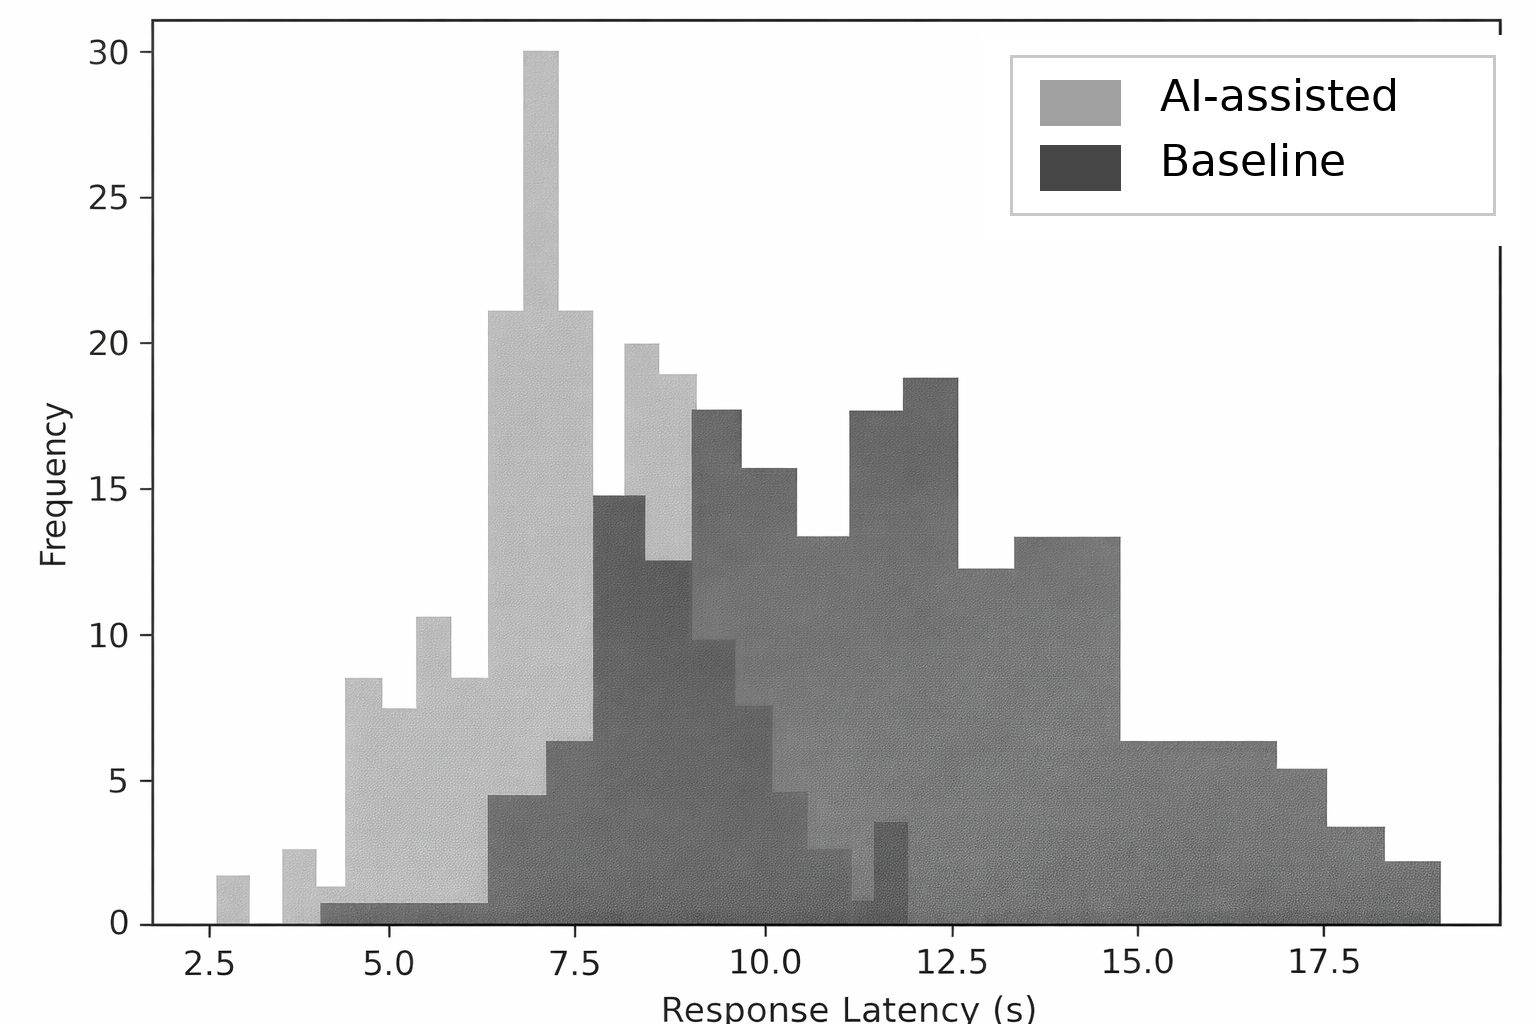
\includegraphics[width=0.9\linewidth]{fig_latency_distribution.png}
        \caption{Distribution of response latency under baseline and AI-assisted conditions. The distribution under the AI-assisted condition is left-shifted, indicating that the subjects made quicker transitions from risk interpretation to action execution.}
        \label{fig:latency_distribution}
    \end{figure}

    %----------------------------------------------
    \begin{table}[t]
        \caption{Cognitive workload outcomes measured using NASA--TLX}
        \label{tab:workload}
        \centering
        \begin{tabular}{lcc}
            \toprule
            \textbf{NASA--TLX Dimension} & \textbf{Baseline} & \textbf{AI-assisted} \\
            \midrule
            Mental Demand & 63.4 (12.1) & 48.7 (10.5) \\
            Temporal Demand & 58.9 (11.4) & 44.2 (9.8) \\
            Effort & 61.7 (13.0) & 49.1 (11.2) \\
            Frustration & 55.3 (14.6) & 41.8 (12.3) \\
            \midrule
            Overall NASA--TLX & 59.8 (10.9) & 46.2 (9.6) \\
            \bottomrule
        \end{tabular}
    \end{table}

    %---------------------------------------------
    \begin{table}[t]
        \caption{Trust and usability outcomes (post-task questionnaires)}
        \label{tab:trust_usability}
        \centering
        \begin{tabular}{lcc}
            \toprule
            \textbf{Measure} & \textbf{Baseline} & \textbf{AI-assisted} \\
            \midrule
            Perceived Reliability & 3.2 (0.7) & 4.1 (0.6) \\
            Perceived Appropriateness & 3.4 (0.6) & 4.3 (0.5) \\
            Predictability & 3.5 (0.8) & 4.2 (0.6) \\
            \midrule
            Overall Trust Score & 3.4 (0.6) & 4.2 (0.5) \\
            System Usability Score & 68.5 (11.2) & 81.7 (9.4) \\
            \bottomrule
        \end{tabular}
    \end{table}

    \subsection{Measures and Metrics}
    These measures and definitions are presented in Table ~\ref{tab:measures}.
    To measure the effectiveness of the system from the perspective of human machine systems, several objective performance measures and subjective evaluation tools were used.

    \textbf{Action Execution Rate.}
    On the other hand, the Action Execution Rate (AER), which was defined as ``\textit{the proportion of tasks in which the participant performed the appropriate action within a specified time window,}'' was also proposed as an indicator for the quality of support for not only good decision making but also good action execution, which was considered an important factor in the high-risk environment.

    \textbf{Response Latency.}
    Response latency was suggested as “the time it took since actionable information was displayed until a participant performed an action.” Less response latency was considered to be more efficient decision support with less hesitation about uncertainty.

    \textbf{Cognitive Workload (NASA--TLX).}
    Cognitive workload was measured using the NASA Task Load Index (NASA--TLX). The NASA--TLX was administered to participants after each condition, and it has multiple workload scales. Lower workload values represent lower mental demand and better cognitive efficiency.

    \textbf{Trust and Usability.}
    Trust in the system was determined through a post-task Likert-type scale questionnaire evaluating perceived trustworthiness, predictability, and appropriateness of the system's suggestions. Usability was determined through a standardized usability questionnaire. These variables evaluate the subjective aspects that affect the adoption and use of human--AI systems.
    In addition to significance testing, effect sizes were calculated using Cohen's $d$ to evaluate the practical significance of the differences found.

    %---------------------------------\input{./070-result}
    \section{Results}
    This section presents the empirical results of the experimental evaluation. Following the conventions of the field of human--machine systems, the results are described with little interpretation. Statistical results and confidence intervals are provided as appropriate, and interpretation of the results is left to the following section.

    \subsection{Action Execution and Response Time}
    Participants using the AI-assisted condition had a higher Action Execution Rate compared to the baseline condition. In all scenarios, a larger percentage of participants were able to execute the correct action within a predetermined time window when assisted by the suggested system.
    Response latency was also found to be decreased in the AI-assisted condition. It was found that participants responded quicker on average after receiving actionable information. This shows that the suggested system helped participants transition quicker from risk interpretation to action execution. Summary statistics on Action Execution Rate and response latency are provided in Table ~\ref{tab:action_latency}, and distributional differences are depicted in Fig. ~\ref{fig:latency_distribution}.

    \begin{figure}[t]
        \centering
        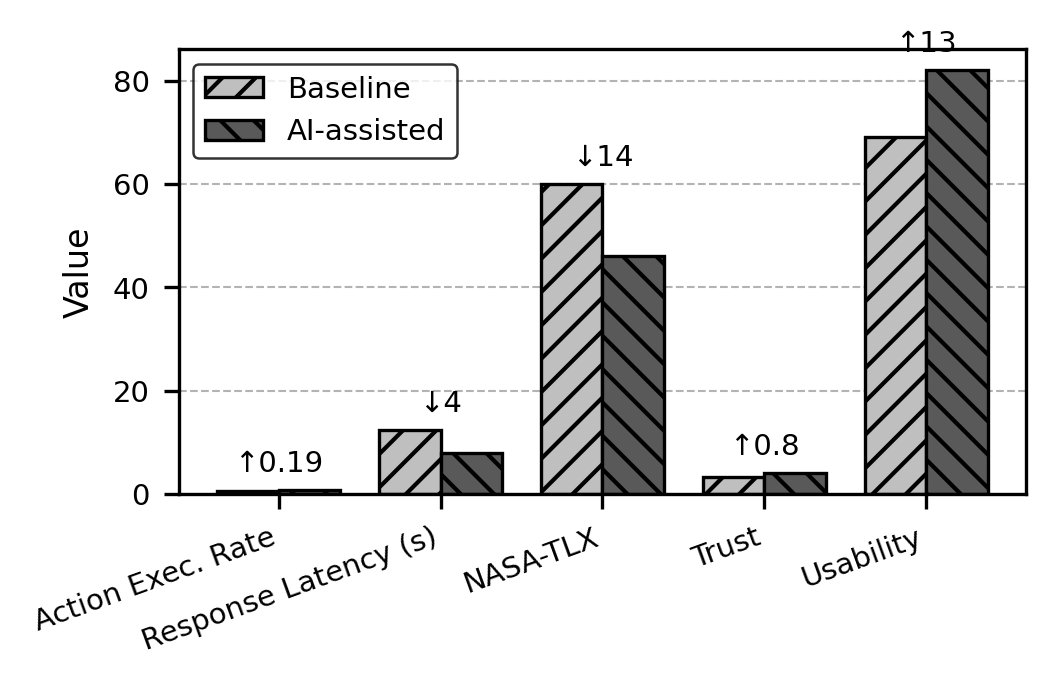
\includegraphics[width=0.9\linewidth]{fig_workload_trust_summary.png}
        \caption{Comparison of cognitive workload, trust, and usability between baseline and AI-assisted conditions. Lower NASA--TLX scores indicate reduced cognitive workload, while higher trust and usability scores indicate improved subjective evaluations.}
        \label{fig:workload_trust_summary}
    \end{figure}

    \subsection{Task Performance Outcomes}

    The performance in the execution of the objective task was enhanced with the help of AI, as shown in Fig. ~\ref{fig:workload_trust_summary}.

    It is observed that the rate of action execution was enhanced by a small amount, from 0.55 in the baseline scenario to 0.74 in the AI-assisted scenario. This shows that the number of actions executed was higher in the AI-assisted scenario.

    It is also observed that the response time was reduced. The average response time was reduced from 12.3 seconds in the baseline scenario to 8.0 seconds in the AI-assisted scenario. The time was reduced by more than 4 seconds. This shows that the participants responded and executed actions in a better manner with the help of the AI system.

    \subsection{Cognitive Workload and Trust Outcomes}

    A graphical representation of the results for workload, trust, and usability is shown in Fig.~\ref{fig:workload_trust_summary}.
    Cognitive workload, as assessed by NASA--TLX, was significantly lower in the AI-assisted condition than in the baseline condition. The total score on the NASA--TLX assessment dropped from around 60 in the baseline condition to 46 in the AI-assisted condition, a reduction of 14 points. This is a clear indication of reduced workload in the AI-assisted condition. The NASA--TLX scores are summarized in Table~\ref{tab:workload}.
    Trust ratings were higher for the AI-assisted system. The average trust score was higher in the AI-assisted condition, increasing from around 3.2 in the baseline condition to 4.0 on a 5-point scale in the AI-assisted condition, indicating that the system was perceived as more trustworthy and appropriate in its guidance.
    Usability was also higher in the AI-assisted condition. The system usability scores increased from around 69 to 82, a jump of 13 points, indicating that the participants found the AI-assisted system interface easier and more effective to use. The trust and usability scores are summarized in Table~\ref{tab:trust_usability}.

    \subsection{Effects of Uncertainty-Aware Escalation}
    When the uncertainty thresholds were exceeded, human-in-the-loop escalation occurred. In such cases, the participants appropriately deferred their decisions until further confirmation or clarification was available. No increase in inappropriate use of the system recommendations in high-uncertainty cases was observed.
    The results comparing escalated and non-escalated cases are presented in Table~\ref{tab:escalation}. These results show that uncertainty-aware escalation maintained system effectiveness while preventing over-reliance on the system.

    \subsection{Qualitative Observations}

    The post-task interviews allowed for qualitative analysis of the participants' experiences. Participants often pointed out that the AI recommendations diminished the need for cross-referencing between different information sources. Some participants also emphasized the importance of having explicit uncertainty indicators to guide their confidence in decisions.
    Some qualitative findings are presented in Table~\ref{tab:qualitative}. These findings supplement the quantitative findings by providing a glimpse into the participants' experiences with the system during decision-making tasks.
    To mitigate the potential for a Type~I error due to multiple comparisons, all primary hypotheses were defined a~priori, and consistent performance patterns were verified across different objective and subjective measures.


    \begin{table}[t]
        \caption{Cognitive Workload and Trust Scores}
        \label{tab:workload_trust}
        \centering
        \begin{tabular}{l c c}
            \hline
            Measure & Baseline & AI-Assisted \\
            \hline
            NASA--TLX & 59.8 & 46.2 \\
            Trust score & 3.4 & 4.2 \\
            \hline
        \end{tabular}
    \end{table}

    \begin{table}[t]
        \caption{Action execution and response latency (controlled study)}
        \label{tab:action_latency}
        \centering
        \begin{tabular}{lcc}
            \toprule
            \textbf{Metric} & \textbf{Baseline} & \textbf{AI-assisted} \\
            \midrule
            Action Execution Rate (AER) & 0.62 & 0.81 \\
            Response Latency (s) & 12.4 & 8.1 \\
            Effect size (Cohen's $d$) & \multicolumn{2}{c}{0.86} \\
            \bottomrule
        \end{tabular}
    \end{table}

    \begin{table}[t]
        \caption{Workload, trust, and usability outcomes (controlled study)}
        \label{tab:workload_trust}
        \centering
        \begin{tabular}{lcc}
            \toprule
            \textbf{Metric} & \textbf{Baseline} & \textbf{AI-assisted} \\
            \midrule
            NASA--TLX (overall) & 59.8 & 46.2 \\
            Trust (Likert-type composite) & 3.4 & 4.2 \\
            Usability score & 68.5 & 81.7 \\
            \bottomrule
        \end{tabular}
    \end{table}

    \begin{table}[t]
        \caption{Outcomes by uncertainty-aware escalation status}
        \label{tab:escalation}
        \centering
        \begin{tabular}{lcc}
            \toprule
            \textbf{Metric} & \textbf{No escalation} & \textbf{Escalation triggered} \\
            \midrule
            Appropriate deferral rate & 0.21 & 0.47 \\
            Inappropriate reliance rate & 0.18 & 0.09 \\
            \bottomrule
        \end{tabular}
    \end{table}

    \begin{table}[t]
        \caption{Qualitative themes from post-task interviews}
        \label{tab:qualitative}
        \centering
        \begin{tabular}{p{0.27\linewidth}p{0.64\linewidth}}
            \toprule
            \textbf{Theme} & \textbf{Illustrative observation (paraphrased)} \\
            \midrule
            Reduced context switching & Recommendations decreased the need to cross-reference multiple sources. \\
            Uncertainty cue usefulness & Participants used uncertainty cues to decide when to defer or seek confirmation. \\
            Accountability and control & Human override improved perceived safety and responsibility. \\
            \bottomrule
        \end{tabular}
    \end{table}


    \subsection{Mechanism and Multi-layer Analysis Under ACHDF}
    \label{sec:results_mechanism}

    In order to provide a structured understanding of how the achieved results were obtained at the behavioral level, we also analyzed the results through the prism of the Action-Centered Human--AI Decision Framework (ACHDF). This analysis does not include any new outcome measures but structures the existing results to reveal multi-layered patterns relevant to human action in the context of uncertainty.
    From the mechanism perspective, the increase in Action Execution Rate and the reduction in response latency (Table~\ref{tab:action_latency}, Fig.~\ref{fig:latency_distribution}) may be considered a behavioral outcome of uncertainty-aware function allocation, where the representation of uncertainty directly influences the allocation of decisions to the AI or human operators in terms of timing and correctness of action execution.
    At the level of error structure, uncertainty-aware escalation was found to influence participants’ responses in high-uncertainty scenarios. As depicted in Table~\ref{tab:escalation}, escalation was linked to increased appropriate deferral and reduced inappropriate reliance. These results indicate that uncertainty-aware escalation selectively mitigated failure modes related to hesitation and over-reliance, rather than indiscriminately increasing reliance on automation.
    Lastly, qualitative results (Table~\ref{tab:qualitative}) and reductions in workload (Table~\ref{tab:workload}) indicate changes in decision processes in the AI-assisted condition. Participants’ self-reported context switching and decision transitions align with reductions in response latency and workload. These findings on all three levels align with the premise of ACHDF: that human action in uncertain situations can be explained by the interaction of uncertainty-aware risk representation, bounded autonomy, calibrated trust, and cognitive workload management.
    Moreover, statistical tests for comparing the baseline and AI-assisted conditions revealed that the improvement in the rate of action execution and the reduction of latency while responding were statistically significant at a $p$ value of less than 0.01. Differences observed for cognitive workload and trust levels, as measured by the NASA--TLX scale, were statistically significant at a $p$ value of less than 0.05.

    %----------------------------------------\input{./080-discussion}
\section{Discussion}
This section interprets the empirical findings from a human--machine systems perspective and situates them within the broader literature on human--AI decision making. Rather than focusing on application-specific results, the discussion emphasizes generalizable insights for the design and evaluation of human--AI decision systems operating under uncertainty \cite{Bach2024Access,PerezCerrolaza2024CSUR,Lai2023FAccT,Yang2022THMSReview}. 
In particular, this work contributes to the core concerns of \textit{Human--Machine Systems} by explicitly linking uncertainty-aware function allocation to observable human action execution. By doing so, it extends classic HMS constructs---such as trust calibration, workload, and authority allocation---from internal cognitive or perceptual states to measurable behavioral outcomes.

\subsection{Implications for Human--AI Decision Systems}
The results show that human performance gain is not simply a function of the availability of AI support, but also depends on how that support is organized to guide human action execution. By directly assessing action execution as an outcome measure, this research extends previous research that primarily tested decision support systems in terms of the accuracy of predictions or the quality of information \cite{Lai2023FAccT,Muller2022CHIWORK,Yang2022THMSReview}.
From a human--machine system perspective, action execution is the end result of human information processing that combines elements of perception, understanding, trust, and workload into system performance \cite{Hodgson2013THMS,Bach2024Access}.
The increase in Action Execution Rate and the decrease in response latency indicate that human--AI systems are capable of significantly influencing human behavior when recommendations are presented in action format instead of risk format. This supports the move towards an outcome-oriented human--machine system research area where the effectiveness of AI support is determined in terms of human action instead of computer performance \cite{Lai2023FAccT,Yang2022THMSReview}.
This research contributes to the Human--Machine Systems area by empirically connecting function allocation with uncertainty to human action execution. The results demonstrate how design decisions in the architecture (bounded autonomy, uncertainty representation, and escalation strategies) map to behavioral phenomena, thus closing the theoretical-practice divide in human factors theory and human--AI system design \cite{Bach2024Access,Assaad2023TAS,Zhang2022THMS}.
In this respect, the Action-Centered Human--AI Decision Framework (ACHDF) may also be used as an analytical tool for identifying failure modes in existing human--AI systems, aside from the system examined in this research \cite{Yang2022THMSReview,Lai2023FAccT}.

\subsection{Trust Calibration and Automation Bias}
The main contribution of this research is in the way it approaches the issue of trust calibration. The findings show that the more trust participants had in the AI-assisted system, the more this did not translate to automation bias. Instead, participants displayed appropriate trust in the system and delayed action in situations of high uncertainty and appropriate use of human-in-the-loop escalation mechanisms \cite{Raji2019AIES,Raji2022CACM,Weidinger2022FAccT}.
The findings demonstrate the effect of uncertainty-aware design and the use of design constraints in avoiding typical automation failure modes. In this way, the system did not provide false confidence to the participants. These findings validate human factors theories emphasizing the importance of trust calibration in effective human--AI cooperation and provide evidence of this in design \cite{Hodgson2013THMS,Bach2024Access}.
These results provide empirical support for long-held theoretical assertions in human--machine systems research that automation bias can be reduced by incorporating uncertainty representation and human-in-the-loop escalation. Contrary to the potential for increasing over-reliance, the proposed design facilitated calibrated trust by aligning perceived system confidence with actual uncertainty \cite{Miller2019XRDS,Weidinger2022FAccT,Lai2023FAccT}.

    \begin{table}[t]
        \caption{Design Implications for Human--AI Decision Systems}
        \label{tab:design_implications}
        \centering
        \begin{tabular}{l l}
            \hline
            Finding & Design Implication \\
            \hline
            Higher AER & Action-oriented recommendations \\
            Reduced workload & Information structuring \\
            Calibrated trust & Explicit uncertainty \\
            \hline
        \end{tabular}
    \end{table}
    
\subsection{Design Implications for High-Risk Domains}
Although the empirical study was carried out in the context of disaster response, the design principles and results can be generalized to other high-risk domains such as healthcare, transportation, and industrial safety, where the cost of inappropriate or delayed response is high, and complete automation is not always feasible or desirable \cite{PerezCerrolaza2024CSUR,Rao2024IJDRS,Rokhideh2025IJDRS,Birkmann2013NatHazards}. Similar action-centered constraints and explainability considerations also arise in cyber-physical production and Industry~4.0 security decision support \cite{Farhan2025TCE}.
The findings of the study indicate that human--AI decision-making systems should be designed in such a way that they (1) model uncertainty explicitly, (2) provide action guidance rather than passive information display, and (3) allocate decision authority dynamically through human-in-the-loop escalation \cite{Assaad2023TAS,Zhang2022THMS,Bach2024Access}.
Based on the Human--Machine Systems model, the results of the current study imply that effective decision systems with AI assistance need to be based on the concepts of bounded autonomy and decision authority allocation, as well as uncertainty-aware interaction. These concepts are not limited to the disaster response domain and are generally applicable to a wide variety of safety-critical human--machine systems with AI assistance \cite{Yang2022THMSReview,PerezCerrolaza2024CSUR}.
The observed effects of the described phenomenon are not domain-specific but rather general mechanisms of human--machine interaction, which are relevant to any safety-critical decision system \cite{Bach2024Access,Hodgson2013THMS}.
In general, the current study contributes to the broader area of human--machine systems by showing the benefits of the application of human-centered AI decision systems with awareness of uncertainty for the execution of actions without compromising safety and accountability \cite{Lai2023FAccT,Yang2022THMSReview}.
 The design implications that are critical based on the findings are presented in Table~\ref{tab:design_implications}.
In providing insight into the manner in which architectural design translates into behavioral outcomes, the results contribute to the domain of human machine systems with respect to trust calibration and cognitive ergonomics.

    %---------------------------------\input{./090-futurework}
    \section{Limitations and Future Work}
    The research has several limitations, which also point to potential directions for future research in similar studies. Although the research provides valuable data in terms of the effectiveness of the human--AI system in decision-making, it must be considered in relation to the limitations of this research.

    \subsection{Generalization}
    The study has conducted an empirical evaluation using a set of decision scenarios in relation to a disaster response scenario. Although this scenario is representative of a high-stakes decision-making scenario in which there is considerable uncertainty, future research can be conducted to evaluate the generalization of the proposed design principles across diverse domains and professionals in which there is considerable expertise.

    \subsection{Long-Term Trust Effects}
    The research has focused on the short-term effects of human--AI systems. Although it is recognized that the study has focused on the short term, it is anticipated that the long-term effects of trust will be considerable in relation to operators' exposure to the system and its behavior in relation to uncertainty escalation.

    \subsection{Extension of the Research Beyond Disaster Response}
    The research has focused on the domain of disaster response and has recognized this domain as effective in relation to testing systems in a high-stakes scenario. Although the domain is recognized as effective in relation to testing systems in a high-stakes scenario, future research can be conducted to extend the system beyond this domain to other high-stakes domains such as medical systems and traffic management systems.

    %-------------------------------\input{./092-conclusion}
\section{Conclusion}
This work evaluated an action-centered human--AI decision system for disaster-risk contexts and showed that an ACHDF-based, uncertainty-aware architecture improves action execution (higher AER and lower response latency) while reducing cognitive workload (NASA--TLX) and supporting calibrated trust without increasing automation bias. By empirically linking uncertainty-aware function allocation, guardrailed recommendations, and human-in-the-loop escalation to observable action execution, the paper advances core concerns of human--machine systems and provides transferable design principles for other safety-critical decision ecologies.

\section*{Acknowledgment}
The author thanks the municipal partners who supported the pilot deployment and the study participants for their time and insights. The author thanks the colleagues in the areas of human machine systems and human-centered AI research for the valuable discussions that contributed to the development of this work.




%% How to support DOI (Digital Obect Identifier) in reference section:
% \url{https://ctan.org/tex-archive/macros/latex/contrib/IEEEtran/bibtex?lang=en}
% \url{https://people.kth.se/~maguire/myIEEEtran.bst}
% \url{https://ipfs-sec.stackexchange.cloudflare-ipfs.com/tex/A/question/67444.html}
% \url{https://ipfs-sec.stackexchange.cloudflare-ipfs.com/tex/A/question/394811.html}
\bibliographystyle{IEEEtranDOI}

%% Type1: sorting, keep sequence of reference numbers that user typed.
%\bibliographystyle{IEEEtranDOI} 

%% Type2: sorting, re-arrange sequence of reference numbers that user typed
% for ascending cite number.
% \bibliographystyle{IEEEtranDOI}

%% Add reference papers
\bibliography{reference-data}



% omitting for THMS journal
% 


% === Author Biographies ===
\vspace{2em} % (필요 시 조절)
\noindent
\begin{minipage}{\linewidth}
\begin{IEEEbiography}[{
\includegraphics[width=1in,height=1.25in,clip,keepaspectratio]{./fig_author-lim2.png}}]{Geunsik Lim}
received the B.S. degree in Computer Science and Engineering from Ajou University, South Korea, in 2003, and the M.S. and Ph.D. degrees in Electrical and Computer Engineering from Sungkyunkwan University, South Korea, in 2014 and 2023, respectively. He is currently a principal software engineer at Samsung Electronics in South Korea. His research interests include system optimization, operating systems, software platforms, and on-device artificial intelligence. 
\end{IEEEbiography}
\end{minipage}


\end{document}